\documentclass[12pt,a4paper,bibliography=totocnumbered]{scrartcl}
\usepackage[ngerman]{babel}

\usepackage{graphicx}
\usepackage{geometry}
%\usepackage{titlesec}
\usepackage{fancyhdr}
\usepackage[pdfpagelabels=true]{hyperref}
\usepackage{xcolor}
\usepackage{listings}
\usepackage[T1]{fontenc}

\definecolor{mGreen}{rgb}{0,0.6,0}
\definecolor{mGray}{rgb}{0.5,0.5,0.5}
\definecolor{airforceblue}{rgb}{0.36, 0.54, 0.66}
\definecolor{amber}{rgb}{1.0, 0.49, 0.0}
\definecolor{coolgrey}{rgb}{0.55, 0.57, 0.67}
\definecolor{davy}{rgb}{0.33, 0.33, 0.33}
\definecolor{backgroundColour}{rgb}{0.95,0.95,0.95}

\lstdefinestyle{CStyle}{
    backgroundcolor=\color{backgroundColour},   
    commentstyle=\color{davy},
    keywordstyle=\color{amber},
    numberstyle=\tiny\color{mGray},
    stringstyle=\color{airforceblue},
    basicstyle=\footnotesize,
    breakatwhitespace=false,         
    breaklines=true,                 
    captionpos=b,                    
    keepspaces=true,                 
    numbers=left,                    
    numbersep=5pt,                  
    showspaces=false,                
    showstringspaces=false,
    showtabs=false,                  
    tabsize=2,
    language=C
}

\geometry{a4paper, top=27mm, left=25mm, right=25mm, bottom=35mm, headsep=10mm, footskip=12mm}

\makeatletter
\renewcommand\@biblabel[1]{}
\makeatother
%__________________________________________________________________

\begin{document}

%\titlespacing{\section}{0pt}{12pt plus 4pt minus 2pt}{-6pt plus 2pt minus 2pt}

% Kopf- und Fusszeile
\pagestyle{fancy}
\renewcommand{\sectionmark}[1]{\markright{\arabic{section}.\ #1}}
\renewcommand{\leftmark}{}
\fancyhf{}
\lhead{}
\chead{}
\rhead{\thesection\space\contentsname}
\lfoot{Abgabe 3}
\cfoot{}
\rfoot{\ \linebreak  \thepage}
\renewcommand{\headrulewidth}{0.4pt}
\renewcommand{\footrulewidth}{0.4pt}

%______________________________________________________________________


%______________________________________________________________________

\clearpage

% Arabische Seitenzahlen
\pagenumbering{arabic}
\setcounter{page}{1}

% Geändertes Format für Seitenränder, arabische Seitenzahlen
\fancyhead[LE,RO]{\rightmark}
%\fancyhead[LO,RE]{\leftmark}
\fancyfoot[LE,RO]{\thepage}

%______________________________________________________________________

\section*{Abgabe 3}

\begin{lstlisting}[style=CStyle]
#include <stdlib.h>
#include <stdio.h>
#include <unistd.h>
#include <time.h>
#include <pthread.h>
#include <sched.h>
#include <string.h>

#define MILLION  1E6


/*
 * Operates for one millisecond
 */
void oneSecMethod() {
	volatile int zero = 0, one = 1, sum;
	int i;
	for (i = 0; i < 50000; i++) {
		sum = zero + one;
	}
	for (i = 0; i < 50000; i++) {
		sum = zero + one;
	}
}

/*
 * Waste the time given in milliseconds
 */
void waste_msecs(unsigned int msecs) {
	int i;
	for (i = 0; i < msecs; i++) {
		oneSecMethod();
	}
}

/*
 * Waste one second and calculates the time waited more than expected
 */
void* function(void* arg) {
	struct timespec start, stop;
	int s, ms, i;

	for (i = 0; i < 10; i++) {
		if (clock_gettime(CLOCK_REALTIME, &start) == -1) {
			perror("clock gettime");
			return (void *) EXIT_FAILURE;
		}

		waste_msecs(1000);

		if (clock_gettime(CLOCK_REALTIME, &stop) == -1) {
			perror("clock gettime");
			return (void *) EXIT_FAILURE;
		}

		usleep(100000);

		s = (stop.tv_sec - start.tv_sec) * 1000;
		ms = (stop.tv_nsec - start.tv_nsec) / MILLION;

		printf("start: %d, n %lu \n", start.tv_sec, start.tv_nsec);
		printf("stop: %d, n %lu \n", stop.tv_sec, stop.tv_nsec);
		printf("Waited miliseconds: %d\n", s + ms);
	}
	return EXIT_SUCCESS;
}

/*
 * Create Thread with highest priority
 * Print priority of thread
 */
int main(int argc, char *argv[]) {
	pthread_t thread_one;
	pthread_attr_t attr;
	struct sched_param param;
	int err;

	param.sched_priority = sched_get_priority_max(SCHED_FIFO);

	pthread_attr_init(&attr);
	// main Thread soll auf diesen Thread warten, damit das Programm erst beendet wird, wenn der Thread mit seiner Berechnung fertig ist. Dadurch wird sichergestellt, dass das Programm immer genau so lange lauft, wie der Thread rechnet und nicht schon vorher beendet wird.
	pthread_attr_setdetachstate(&attr, PTHREAD_CREATE_JOINABLE);
	pthread_attr_setschedparam(&attr, &param);

	err = pthread_attr_setinheritsched(&attr, PTHREAD_EXPLICIT_SCHED);

	if (err != 0) {
		printf("pthread_attr_setinheritsched: %s ", strerror(err));
	}

	err = pthread_create(&thread_one, &attr, &function, NULL);

	if (err != 0) {
		printf("pthread_create: %s ", strerror(err));
	}

	pthread_attr_getschedparam(&attr, &param);

	printf("Thread Priority: %d\n", param.sched_priority);

	err = pthread_join(thread_one, NULL);

	if (err != 0) {
		printf("pthread_create: %s ", strerror(err));
	}

	return EXIT_SUCCESS;
}
\end{lstlisting}

\newpage
\begin{figure}[h]
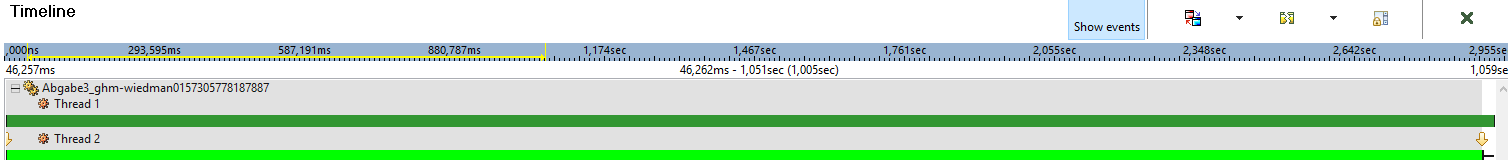
\includegraphics[width=\textwidth]{bilder/QNX_Abgabe3_HeavyWork}
\centering
\end{figure}
Wie in der Messung zu sehen ist, wird genau eine Sekunde gerechnet.
%______________________________________________________________________

\end{document}












